\documentclass[fleqn,usenatbib]{mnras}
\usepackage[T1]{fontenc}
\usepackage{graphicx,amsmath,booktabs,xcolor}
\newcommand{\pending}[1]{\textcolor{red}{[#1]}}
\newcommand{\RecallMsixOOF}{0.47 [0.25, 0.66]}
\newcommand{\RecallGBMOOF}{0.25 [0.20, 0.30]}
\newcommand{\DiffOOF}{+0.22 [+0.04, +0.38]}
\newcommand{\PalignMedian}{1.8\%}
\newcommand{\NexpCHIME}{$5.3\times10^{-6}$}
\newcommand{\NexpCHIMEbias}{$1.2\times10^{-4}$}
\newcommand{\GainAllSky}{$\sim$50}
\newcommand{\GainTenYr}{1.4--1.8}
\newcommand{\HostSens}{$-$19\%}
\newcommand{\HostSensTau}{$-$13\%}
\newcommand{\NexpEcho}{$3.2\times10^{-5}$}
\newcommand{\NexpEchoPair}{$1.5\times10^{-5}$}
\newcommand{\FarHeldOut}{1 of 166{,}000 held-out scrambles}
\newcommand{\FarRateUp}{$2.9\times10^{-5}$}
\newcommand{\FarSearchUp}{0.002}
\newcommand{\ReproHashes}{7/7 match}
\newcommand{\ReproMsix}{0.668}
\newcommand{\SthreeFPRMsix}{1.4\% [0.1, 4.0]}
\newcommand{\SthreeFPRGBM}{1.3\% [0.2, 2.8]}
\newcommand{\SthreeTwinMsix}{0.76 against 0.87}
\newcommand{\SthreeTwinGBM}{0.83 against 0.83}
\newcommand{\EhSim}{1.94}
\newcommand{\EhReal}{1.10 [0.20, 2.55]}
\newcommand{\SthreeFPRMsixSeeds}{1.4, 1.9, 1.6\%}
\newcommand{\SthreeFPRMsixHi}{5\%}
\newcommand{\GapMsix}{+0.6 to +1.2 points}
\newcommand{\GapBaseMax}{0.5 points}
\newcommand{\BoneLowReal}{6.2, 3.8, 2.4\%}
\newcommand{\BoneLowTwin}{5.6, 4.0, 2.5\%}
\newcommand{\SnrLowReal}{16.9}
\newcommand{\SnrLowSim}{13.5}
\newcommand{\EhSimSeeds}{1.9, 1.7, 7.3}
\newcommand{\EhRealSeeds}{1.10, 1.86, 1.53}
\newcommand{\ReproSeeds}{0.668 / 0.649 / 0.616}
\newcommand{\AblSeeds}{3}
\newcommand{\AblFull}{0.644}
\newcommand{\AblNoalign}{0.557, difference $-$0.087 [$-$0.186, $-$0.025]}
\newcommand{\AblHardneg}{0.698, difference +0.053 [$-$0.011, +0.082]}
\newcommand{\AblNoimp}{0.474, difference $-$0.170 [$-$0.254, $-$0.052]}
\newcommand{\ForecastRows}{CHIME, Catalog 2 & $2.9\times10^{-3}$ & $5.3\times10^{-6}$ & $3.2\times10^{-5}$ \\
All-sky, same sources & $2.9\times10^{-3}$ & $2.6\times10^{-4}$ & $6.3\times10^{-4}$ \\
CHIME, Catalog 2, $\gamma=1.5$ & $1.8\times10^{-2}$ & $1.2\times10^{-4}$ & $4.9\times10^{-4}$ \\
All-sky, same sources, $\gamma=1.5$ & $1.8\times10^{-2}$ & $6.1\times10^{-3}$ & $9.3\times10^{-3}$ \\
CHIME-like, 10 yr & $2.8\times10^{-3}$ & $7.4\times10^{-6}$ & $4.9\times10^{-5}$ \\
All-sky, 10 yr & $2.8\times10^{-3}$ & $3.7\times10^{-4}$ & $6.8\times10^{-4}$ \\
CHIME-like, 10 yr, $\gamma=1.5$ & $1.8\times10^{-2}$ & $2.2\times10^{-4}$ & $6.3\times10^{-4}$ \\
All-sky, 10 yr, $\gamma=1.5$ & $1.8\times10^{-2}$ & $7.4\times10^{-3}$ & $9.6\times10^{-3}$ \\}


\title[Identifying lensed repeating FRBs]{A Siamese network for identifying gravitationally lensed repeating fast radio bursts:
benchmark, transit geometry and forecasts for CHIME/FRB Catalog~2 and all-sky monitors}
\author[Draft]{Draft authors \thanks{Draft generated from the project repository; not for circulation.}\\
Affiliations to be added}
\date{Draft \today}
\pubyear{2026}

\begin{document}
\label{firstpage}
\pagerange{\pageref{firstpage}--\pageref{lastpage}}
\maketitle

\begin{abstract}
A galaxy-lensed repeating fast radio burst (FRB) would repeat every burst after a fixed delay of days to months,
and the two copies of a burst would differ only by propagation effects.
We build semi-synthetic lensed repeaters from the 981 public dynamic spectra of the 83 repeaters in CHIME/FRB Catalog~2,
with real off-pulse noise, measured injection S/N and per-image scattering, scintillation and residual dispersion, plus
\emph{impostor} pairs of different bursts that share a plasma-lens envelope or a scintillation pattern.
On this benchmark a Siamese encoder with a correlation layer and feature-map fusion recovers
\RecallMsixOOF\ of lensed pairs at 1\% false-positive rate in source-grouped cross-validation, against \RecallGBMOOF\
for the best physics- or feature-based baseline (paired difference \DiffOOF; development data, test split unopened).
Its residual false positives are almost all envelope-sharing impostors, and ablations show that both the alignment layer
and training on impostors are needed. On real cross-source pairs, which are true negatives, its false-positive rate at
the simulated 1\% threshold is \SthreeFPRMsixSeeds\ over three seeds, within the pre-registered 2\% limit; re-simulating
each real pair shows a small genuine sim-to-real gap for the learned model only, which grows with the energy the templates miss. An independent reproduction regenerates all frozen sets bit for bit.
At the source level, the delay of a lens is constant to far better than the 4\,ms catalogue timing, so two burst
pairs sharing one delay are already significant for all but the most active repeaters.
However, a transit telescope sees a burst only within minutes of transit, so the copy of every recorded burst lands at
the same hour angle: copies are recorded only if the delay is within minutes of a whole number of sidereal days.
This happens for \PalignMedian\ of lens delays at the median declination of the sample, so lensed repeaters do
\emph{not} escape the transit problem that limits one-off FRBs.
For Catalog~2 we expect \NexpCHIMEbias\ detectable lensed repeaters (\NexpCHIME\ without magnification bias),
and an all-sky monitor watching the same sources would gain a factor \GainAllSky; a longer transit survey would not.
\end{abstract}

\begin{keywords}
fast radio bursts -- gravitational lensing: strong -- methods: data analysis -- methods: statistical
\end{keywords}

\section{Introduction}
Strongly lensed FRBs have been proposed as probes of compact dark matter \citep{Kader2022,Leung2022,Krochek2022} and,
for galaxy lenses with delays of days to months, of cosmology through precise time delays \citep{Li2018,Wucknitz2021}.
No lensed FRB is confirmed; the strongest candidate is a 3.4$\sigma$ millisecond-scale double burst in Catalog~1 \citep{Chang2024}.
For one-off FRBs a transit instrument such as CHIME rarely records both images of a galaxy lens:
the second image must arrive while the source is again in the beam \citep{ConnorRavi2022}.
Repeating FRBs have been argued to avoid this, because both image streams keep firing over years of exposure.

Two questions decide whether a search of the CHIME/FRB Catalog~2 repeaters is useful.
First, can the morphology of two bursts tell a lensed copy from a different burst of the same source,
including impostors that share a propagation imprint?
Second, how often are both copies of a burst recorded at all?
Machine-learning work on FRBs has so far classified repeaters against non-repeaters; lensed-pair classifiers exist for
gravitational waves \citep{Goyal2021,Zhang2026} but not for FRBs.
We answer both questions with real CHIME data wherever it exists and simulation only for the lensing itself.
Our contributions are: (i) a semi-synthetic benchmark of lensed, repeat, unrelated and impostor burst pairs built from all
981 public Catalog~2 repeater spectra, with a ladder of physics, feature and learned methods; (ii) a transfer check on real
true-negative pairs in which per-pair twin re-simulation separates genuine sim-to-real gaps from sample composition;
(iii) a source-level timing test with a held-out false-alarm calibration; (iv) the transit-alignment argument, verified
by simulation against the analytic window width, which shows that lensed repeaters do not escape the transit problem;
and (v) forecasts for Catalog~2, a longer survey and an all-sky monitor. All development results were reproduced on a
second machine, and the test split remains sealed under a pre-registered blind protocol.

\section{Data}
\label{sec:data}
We use the Stokes-I dynamic spectra of all 981 repeater bursts (83 sources) in CHIME/FRB Catalog~2
\citep{CHIME2025cat2}, at 0.983\,ms and 400--800\,MHz.
Each burst is binned to $256$ channels $\times\,160$ samples, centred on the catalogue emission region, and normalised by
its off-pulse statistics; six bursts at coarser time resolution are excluded as templates.
The fitburst models of the bursts serve as noise-free templates. They miss a median 35\% of the on-pulse signal energy,
which lowers the similarity of simulated pairs of every kind by a near-constant $\sim$8\% relative to real pairs in a
twin test, while for the cross-correlation baseline the simulated rank correlation with real pairs reaches the
simulation-to-simulation noise ceiling in every S/N bin (the learned model does not; Section~\ref{sec:trackb}). Absolute thresholds therefore come from real negatives only.
Sources are split 60/20/20 into train/validation/test by burst count, with the two most active repeaters forced into training.
An independent reproduction on a second machine, which re-downloaded and re-processed all 981 spectra, rebuilt the
injection cache with the same counts (950 eligible templates, 856 backgrounds) and regenerated the frozen validation
and grouped-fold sets: hashes \ReproHashes.

\section{Semi-synthetic lensed pairs}
\label{sec:pairs}
A pair is one of four classes. A \emph{lensed} pair places the same template twice; a \emph{repeat} pair places two
different templates of one source; an \emph{unrelated} pair takes templates from two sources; an \emph{impostor} pair
places two different templates of one source that share either a smoothed spectral envelope (I1, a plasma-lens caustic),
a scintillation pattern (I2), or both.
Each member is injected at a measured matched-filter S/N on a real off-pulse background from another burst, with its own
time shift ($\pm10$ samples), residual DM, scattering and scintillation; flux ratios are drawn so that they carry no information.
Frozen validation and test sets of 4000 pairs and bright sets with pair minimum S/N\,$\ge25$ (the pre-specified headline bin)
are hashed so that any change of code or inputs is detected.

\section{Methods}
\label{sec:methods}
\subsection{Benchmark ladder}
All methods score the same pairs, averaged over both member orders:
(1) cross-correlation within the on-pulse box, maximised over lags and common channels;
(2) a physics statistic fitting one member to the other convolved with a scattering kernel over $\mu$, lag, $\Delta$DM and
scattering grids;
(3) gradient-boosted trees on seven pixel-measured burst properties;
(4) a two-channel CNN;
(5) a classic Siamese network (vector embeddings);
(6) a Siamese encoder whose feature maps are aligned by a correlation layer over $\pm24$ samples and fused as
$|g(A)-g(B)|$ and $g(A)\cdot g(B)$ (primary);
(7) cross-attention between time--frequency patches.
Learned models are trained on pairs generated on the fly from training sources with a four-class cross-entropy.

\subsection{Metric and comparison}
The primary metric is recall of lensed pairs at 1\% false-positive rate against repeat and impostor pairs, with a
source-level bootstrap in which thresholds are recomputed in every resample. Because the validation CI was wide, the
pre-registered rule switched the primary comparison to five source-grouped folds before the test split is opened.

\subsection{Source-level timing (Track C)}
\label{sec:trackc}
A lens repeats every burst after one delay $\Delta t$. Catalogue arrival times referenced to infinite frequency have a
median uncertainty of 4\,ms, so pairs $(i,j)$ and $(k,l)$ of one source share a delay if
$|\Delta t_{ij}-\Delta t_{kl}|<4\sqrt{\sigma_{ij}^2+\sigma_{kl}^2}$ and their S/N ratios agree within a factor 2.
The statistic $k_{\max}$ is the largest set of disjoint pairs sharing a delay.
Its background comes from time-scrambled burst lists, in which every burst moves by a random whole number of sidereal days;
this keeps hour angles, S/N and the transit selection. The unscrambled lists are never scored before unblinding.
Each source's threshold $k_{\rm thr}$ is the smallest $k\ge2$ whose background probability is at most $10^{-3}$, set
from 2000 scrambles. Efficiencies come from lensed copies injected into scrambled lists.

\subsection{Lens population and observation}
Galaxy lenses are singular isothermal spheres with the velocity-dispersion function of \citet{Choi2007}.
Source redshifts come from host galaxies for seven localised repeaters and otherwise from the NE2001 DM excess through
the Macquart relation \citep{Macquart2020}, with halo and host contributions.
For each lens, $\Delta t = 2y\theta_{\rm E}^2(1+z_{\rm l})D_{\rm l}D_{\rm s}/(cD_{\rm ls})$ and the trailing image is fainter
by $r=(1-y)/(1+y)$.
A copy is recorded if it falls within $|{\rm HA}|\cos\delta<1.1^\circ$ of upper transit (or lower transit for
$\delta>70^\circ$), inside the survey, on an observing day (from the catalogue exposure), and above S/N\,10.
The transit window was measured from the real bursts: 99\% of them lie within $1.08^\circ$ of transit.

\section{Results}
\subsection{Pair classification}
\label{sec:trackb}
Table~\ref{tab:trackb} and Fig.~\ref{fig:trackb} summarise the development results.
\begin{figure}
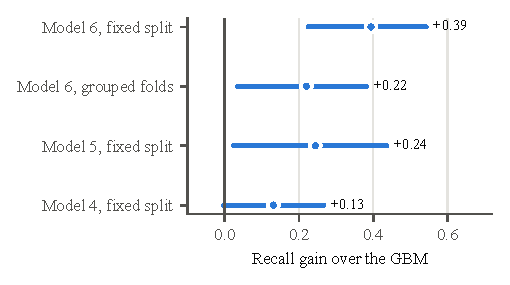
\includegraphics[width=\columnwidth]{fig_trackb.pdf}
\caption{Paired recall gain over the feature GBM at 1\% FPR (S/N\,$\ge25$), with 95\% source-bootstrap intervals
(development data; fixed split: three seeds; grouped folds: out-of-fold).}
\label{fig:trackb}
\end{figure}
Model~6 leads every other method on the fixed validation split and in grouped folds. Replicates on a second machine
reach \ReproSeeds\ (Table~\ref{tab:trackb}), about 0.05 below the original seeds but still far above the GBM.
Its false positives at the 1\% threshold are almost all I1 impostors (shared spectral envelope); I2 impostors and plain
repeats are rarely confused. One two-burst source sets the threshold of one fold, because its few repeat and impostor
pairs look alike to the model, which widens the out-of-fold interval.

\begin{table*}
\caption{Recall at 1\% FPR, lensed vs repeat + impostor, S/N\,$\ge25$, development data. Brackets: 95\% source bootstrap.}
\label{tab:trackb}
\begin{tabular}{lcc}
\toprule
Method & Fixed split (3 seeds) & Grouped folds (OOF) \\
\midrule
Feature GBM (best of 1--3) & 0.285 [0.180, 0.401] & 0.246 [0.199, 0.297] \\
Model 6 (correlation + fusion) & 0.701 / 0.698 / 0.684 & 0.467 [0.253, 0.662] \\
Model 5 (classic Siamese) & 0.500 / 0.559 / 0.541 & -- \\
Model 4 (two-channel CNN) & 0.423 / 0.409 / 0.407 & -- \\
Model 7 (cross-attention) & 0.471 / 0.013 / 0.579 & -- \\
Model 6 $-$ GBM & +0.394 [+0.226, +0.542] & +0.220 [+0.035, +0.381] \\
\midrule
Model 6, independent replicate$^a$ & \ReproSeeds & -- \\
\bottomrule
\end{tabular}
\par\smallskip\noindent{\footnotesize $^a$Second machine, seeds 0/1/2, 4 data workers instead of 14, which changes the training pair stream. The pre-registered
range 0.66--0.72 applied to seed~0 (passed); seeds 1 and 2 fall below it, so this machine's replicates sit about 0.05 below
the original seeds.}
\end{table*}

\paragraph*{Transfer to real data.}
Cross-source pairs of real bursts are true negatives, so they can be scored without unblinding. Among the 89 validation
bursts of 26 sources there are 3750 such pairs. For each method and bin of pair minimum S/N and mask overlap we set the
threshold at 1\% FPR on 20\,000 generic simulated unrelated pairs from the same sources, and measured the real rate above
it (pre-registered criterion: at most 2\%). In the headline bin (793 real pairs) every method passes
(Fig.~\ref{fig:stage3}): the real FPR is \SthreeFPRMsix\ for model~6 (\SthreeFPRMsixSeeds\ for seeds 0, 1, 2; intervals
reach \SthreeFPRMsixHi) and \SthreeFPRGBM\ for the GBM (95\% source bootstrap). Two cells fail. Cross-correlation exceeds
2\% below S/N\,25 (\BoneLowReal\ for the three block sizes), and in the S/N\,$\ge50$ bin (85 real pairs) several methods
exceed it in point estimate through the same two pairs, both involving the bright bursts of FRB~20220428C.

\paragraph*{Transfer versus composition.}
A real-negative rate can differ from 1\% for two reasons: the simulator misses something (a transfer gap), or the real
pairs are a different mix of templates and S/N from the generic simulated pairs (composition). The twins separate the two:
each real pair is re-simulated twice from its own two templates at its own S/N, so at the same threshold the real-minus-twin
rate is the transfer gap and the twin rate minus 1\% is the composition effect. For every baseline the transfer gap is
consistent with zero in every bin (at most \GapBaseMax\ in the headline bin). The cross-correlation failure below S/N\,25 is
pure composition: its twins exceed the threshold as often as the real pairs (\BoneLowTwin), because real pairs in that bin
are brighter (median S/N \SnrLowReal\ against \SnrLowSim) and the cross-correlation grows with S/N within the bin.
Model~6 is the one method with a genuine gap, \GapMsix\ in the headline bin across seeds, with intervals touching zero.
The rank form of the twin test agrees: model~6's rank correlation with its twins falls short of the twin-to-twin ceiling
(\SthreeTwinMsix) while the GBM's reaches it (\SthreeTwinGBM). The gap grows with the share of on-pulse energy the
templates miss. Measuring each burst's deficit as $1-s^2/E_{\rm on}$, with $s$ the template's matched-filter S/N in the
data and $E_{\rm on}$ the on-pulse signal energy (median 0.18 for the validation bursts; this matched-filter measure is smaller than the residual-energy figure of Section~\ref{sec:data}), the per-pair deficit correlates
with model~6's real-minus-twin score (Spearman $\rho=0.16$--$0.23$ over seeds, against $\le0.05$ for every baseline) and
with its rank discrepancy ($\rho=0.13$--$0.24$). The learned model thus reads structure that the
templates lack, as feared, but the cost so far is about one point of false-positive rate, inside the limit. We suggest that
transfer checks report the twin-matched gap alongside the raw rate, since the raw rate confounds the two effects.

\begin{figure}
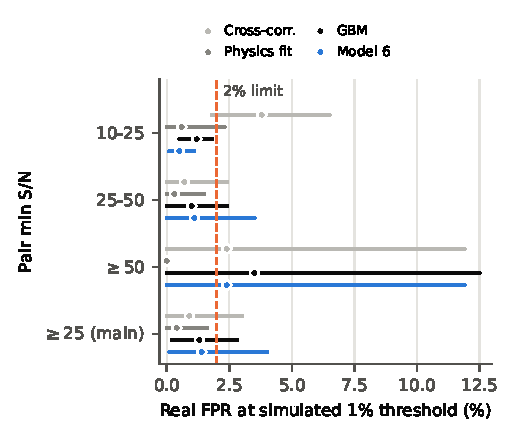
\includegraphics[width=\columnwidth]{fig_stage3.pdf}
\caption{Stage~3 transfer check on validation sources: share of real cross-source pairs (true negatives) above each method's
threshold at 1\% FPR on simulated unrelated pairs (model~6: seed~0; blocks of size 4 for the baselines), by pair minimum S/N (`main': the pre-registered S/N\,$\ge25$ bin), with 95\% source-bootstrap intervals. Dashed: the
pre-registered 2\% limit.}
\label{fig:stage3}
\end{figure}

\paragraph*{Ablations.}
Each ablation retrains model~6 on this machine and is compared with the full model trained with the same seeds
(\AblSeeds\ per configuration; full model \AblFull), as seed-mean recall on the validation bright set with paired
source-bootstrap intervals.
Removing the correlation layer, so that feature maps are fused without alignment, gives recall \AblNoalign.
Removing impostors from training gives \AblNoimp: without them the network mistakes envelope-sharing bursts of one source
for lensed copies. Oversampling hard repeat negatives (the most template-similar of four draws) gives \AblHardneg:
a small gain in every seed whose interval still includes zero. Hard-negative training also biases a learned likelihood
ratio (Appendix~\ref{app:lr}), so we do not adopt it without a correction.
The two design choices that distinguish model~6, alignment and an impostor class, are thus both needed.

\subsection{Timing false-alarm rate}
To check the thresholds, we recomputed every $k_{\rm thr}$ from one random stream and counted exceedances in 2000 fresh
scrambles per source from an independent stream. We found \FarHeldOut\ (95\% upper limit \FarRateUp\ per source and list),
or at most \FarSearchUp\ false sources in a search of all 83 repeaters. The test is conservative because $k$ is an integer:
for most sources no scramble reaches even $k=2$. Only the most active repeater, FRB~20220912A (373 bursts), reaches $k=2$ in
every scramble and needs $k_{\rm thr}=4$.

\subsection{Transit geometry}
\label{sec:transit}
Every burst that CHIME records arrives within minutes of transit. Its copy arrives $\Delta t$ later, at hour angle
${\rm HA}+24\,{\rm h}\times{\rm frac}(\Delta t/T_{\rm sid})$, the \emph{same} offset for every burst of the source.
Copies are therefore recorded for all bursts or for none, and only if $\Delta t$ lies within a few minutes of a whole
number of sidereal days. Over the SIS delay distribution this happens for a fraction $p_{\rm align}$ of lenses
(median \PalignMedian\ over the 83 sources; higher near the pole, where the window widens and lower transits add a chance
near half a sidereal day). A repeater thus offers many pairs \emph{once aligned}, but the chance of alignment is the same
$\sim\theta_{\rm EW}/2\pi$ that limits one-off FRBs \citep{ConnorRavi2022}.
This corrects the assumption that lensed repeaters escape the transit problem.
Fig.~\ref{fig:transit} shows that the simulated $p_{\rm align}$ follows the width of two transit windows per sidereal day,
the analytic expectation when the recorded bursts spread across one window.
\begin{figure}
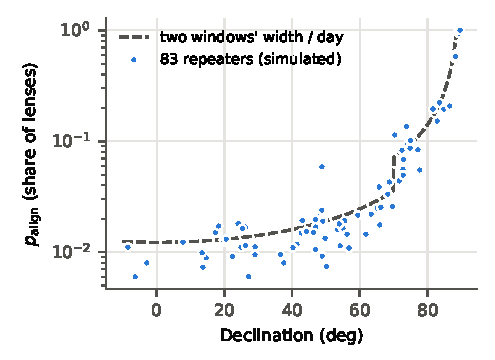
\includegraphics[width=\columnwidth]{fig_transit.pdf}
\caption{Share of SIS lens delays for which CHIME records the copies of a repeater's bursts, against declination.
Points: the 83 Catalog~2 repeaters with their own burst hour angles, exposure and redshift. Dashed: twice the transit-window
width per sidereal day (doubled again above $70^\circ$, where lower transits add a window).}
\label{fig:transit}
\end{figure}

\subsection{Forecasts}
\label{sec:forecast}
Table~\ref{tab:forecast} gives the expected number of lensed repeaters whose timing statistic exceeds a per-source
false-alarm probability of $10^{-3}$, and the number with at least one recorded copy (a candidate for the pair classifier).
\begin{table}
\caption{Expected lensed repeaters in the Catalog~2 sample. $\gamma$: magnification-bias slope of the integral counts.}
\label{tab:forecast}
\resizebox{\columnwidth}{!}{%
\begin{tabular}{lccc}
\toprule
Survey & $\sum\tau$ & $N_{\rm exp}$ (timing) & $N_{\rm exp}$ ($\ge1$ copy) \\
\midrule
\ForecastRows
\bottomrule
\end{tabular}}
\end{table}
Fig.~\ref{fig:forecast} compares CHIME with an all-sky monitor watching the same sources.
\begin{figure}
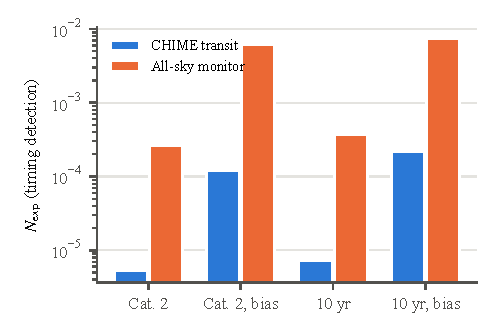
\includegraphics[width=\columnwidth]{fig_forecast.pdf}
\caption{Expected timing detections in the Catalog~2 repeater sample, for the survey as observed and stretched to 10 years,
without and with magnification bias ($\gamma=1.5$).}
\label{fig:forecast}
\end{figure}
A null result in Catalog~2 is therefore expected, and the search serves as a demonstration and a check of the false-alarm rate.
Stretching the same transit survey to 10 years raises $N_{\rm exp}$ by only a factor \GainTenYr: a longer baseline admits
longer delays and more bursts, but leaves the alignment requirement unchanged. An all-sky monitor watching the same sources
gains a factor \GainAllSky. For CHIME-like surveys the limit is sky coverage, not time on sky.

\section{Discussion}
\paragraph*{What the classifier can and cannot claim.}
Simulated false-positive rates rank methods only; thresholds for a search come from real negatives (cross-source pairs and
time-scrambled lists). The lensed class has no real counterpart, so its realism rests on the twin tests and the template-deficit
argument, which makes simulated lensed pairs \emph{less} alike than real ones would be.

\paragraph*{From scores to evidence.}
Posterior odds for a candidate are a likelihood ratio times prior odds from $\tau$.
On a closed-form benchmark (Appendix~\ref{app:lr}) we find that an uncorrected hard-negative training scheme biases a learned
likelihood ratio low by about 1\,dex, that a misspecified repeat-similarity prior raises the false-positive rate about
12-fold at a fixed threshold, and that the identity $E_{H_0}[r]\le1$ can be tested on known negatives alone with a betting
e-process \citep{WaudbySmith2024,Ramdas2024}.
We applied the identity to model~6, taking $\hat r=\exp(\ell_{\rm lensed}-\ell_{\rm unrelated})$ from its balanced-class logits.
On simulated unrelated pairs the mean of $\hat r$ is \EhSimSeeds\ for seeds 0, 1, 2 (seed~0: bootstrap 1.42--2.61), so
the network over-claims evidence by a factor of about two or more, driven by a handful of pairs in the tail. On the 3750 real
cross-source pairs the means are \EhRealSeeds\ (seed~0: \EhReal, source bootstrap), consistent with 1 within a factor of
two: real negatives show no extra over-claiming. The betting test has little power here, because $\hat r$ is heavy-tailed
(the ten largest values carry about half the sum), so we report the bootstrap. A factor-of-a-few bias in $\hat r$ is small
against the uncertainty of $\tau$, but a posterior for any candidate should calibrate $\hat r$ on real negatives first.

\paragraph*{Implications for future surveys.}
An all-sky monitor removes the alignment requirement, and a longer transit survey does not
(Section~\ref{sec:forecast}). Arrays with wide, continuous fields of view, such as the proposed BURSTT \citep{Ho2023}, are
therefore the natural place for repeater-timing searches. A rate per year for such an array needs its own repeater
population and exposure and is beyond this paper; the per-source efficiencies we publish allow it to be computed.
For transit instruments the pair classifier keeps a role that timing cannot fill: a single recorded copy of a single burst,
which can occur even when no timing pattern forms. In the Catalog~2 sample we expect \NexpEcho\ lensed repeaters with at
least one recorded copy, about six times the timing yield; at the development recall of model~6 the pair channel would
find \NexpEchoPair. Both channels are far below one for CHIME, so the classifier's value lies in surveys with continuous
sky coverage and in vetting candidates, where its false positives (envelope-sharing impostors) are the relevant background.

\paragraph*{Limitations.}
(i) All classification numbers are development results; the test split stays sealed until the team signs off the
propagation model. (ii) Lenses are singular isothermal spheres without shear, so four-image systems and shear-induced
delay spreads are absent; the transit argument depends only on the delay, not on the lens model. (iii) Redshifts of the 76
unlocalised repeaters come from DM, and a few high-DM sources dominate $\sum\tau$; a large host DM would bias them high.
Raising the median host DM from 68 to 150\,pc\,cm$^{-3}$ changes $\sum\tau$ by \HostSensTau\ and the CHIME timing yield by
\HostSens, so the forecasts are not sensitive to it. (iv) The magnification-bias slope of CHIME repeaters is unmeasured, which is why we bracket it.
(v) Observing days are drawn from the integrated exposure, assuming downtime spread evenly over the survey.
(vi) The Stage~3 check uses 26 validation sources, so its S/N\,$\ge50$ bin is small.

\section{Conclusions}
\begin{enumerate}
\item On semi-synthetic pairs built from all public Catalog~2 repeater spectra, a Siamese encoder with a correlation
layer and feature-map fusion separates lensed copies from other bursts of the same source better than physics and feature
baselines: recall \RecallMsixOOF\ against \RecallGBMOOF\ at 1\% FPR in source-grouped folds (development data).
Envelope-sharing impostors are the remaining confusion. On real cross-source negatives its false-positive rate at the
simulated 1\% threshold is \SthreeFPRMsixSeeds\ over three seeds, within the pre-registered limit. Twin re-simulation
separates a small genuine transfer gap (\GapMsix, model~6 only) from composition effects, which explain the one baseline
failure; search thresholds must come from real negatives.
\item A galaxy lens fixes the delay to far better than the catalogue timing, so two burst pairs sharing one delay are
already a detection for all but the most active repeaters. Held-out scrambles confirm the false-alarm rate is
conservative: at most \FarSearchUp\ false sources in a search of all 83 repeaters.
\item A transit instrument records the copies of a repeater's bursts only if the delay is within minutes of a whole
number of sidereal days, which happens for \PalignMedian\ of lenses at the median. Lensed repeaters therefore do not
escape the transit problem of one-off FRBs.
\item The Catalog~2 sample is expected to contain \NexpCHIME--\NexpCHIMEbias\ detectable lensed repeaters, so a null
search is expected. A longer transit survey changes this little; an all-sky monitor gains a factor \GainAllSky.
\end{enumerate}
\pending{Test-split and search results, after team sign-off under the blind protocol.}

\section*{Data Availability}
All inputs are public (CHIME/FRB Catalog~2, DOI 10.11570/25.0066). Code, frozen manifests and hashes are in the project repository.

\bibliographystyle{mnras}
\bibliography{references}

\appendix
\section{Reference likelihood ratios on a closed-form benchmark}
\label{app:lr}
A linear-Gaussian pair simulator with an exact marginal likelihood ratio (lensed: correlation $\rho=1$ between the intrinsic
shapes; repeat: $\rho<1$ drawn from a prior) tests neural ratio estimators against the truth on 2.4 million pairs.
Standard training is self-calibrated in the tail and loses power instead; doubling the training budget recovers much of it.
Oversampling similar negatives without correction under-claims by about 1\,dex at every budget, while importance weighting
or conditioning on $\rho$ and re-marginalising preserve calibration. Full results: update 2026-11-07 in the repository.

\bsp
\label{lastpage}
\end{document}
